\documentclass{article}\usepackage[]{graphicx}\usepackage[]{color}
% maxwidth is the original width if it is less than linewidth
% otherwise use linewidth (to make sure the graphics do not exceed the margin)
\makeatletter
\def\maxwidth{ %
  \ifdim\Gin@nat@width>\linewidth
    \linewidth
  \else
    \Gin@nat@width
  \fi
}
\makeatother

\definecolor{fgcolor}{rgb}{0.345, 0.345, 0.345}
\newcommand{\hlnum}[1]{\textcolor[rgb]{0.686,0.059,0.569}{#1}}%
\newcommand{\hlstr}[1]{\textcolor[rgb]{0.192,0.494,0.8}{#1}}%
\newcommand{\hlcom}[1]{\textcolor[rgb]{0.678,0.584,0.686}{\textit{#1}}}%
\newcommand{\hlopt}[1]{\textcolor[rgb]{0,0,0}{#1}}%
\newcommand{\hlstd}[1]{\textcolor[rgb]{0.345,0.345,0.345}{#1}}%
\newcommand{\hlkwa}[1]{\textcolor[rgb]{0.161,0.373,0.58}{\textbf{#1}}}%
\newcommand{\hlkwb}[1]{\textcolor[rgb]{0.69,0.353,0.396}{#1}}%
\newcommand{\hlkwc}[1]{\textcolor[rgb]{0.333,0.667,0.333}{#1}}%
\newcommand{\hlkwd}[1]{\textcolor[rgb]{0.737,0.353,0.396}{\textbf{#1}}}%
\let\hlipl\hlkwb

\usepackage{framed}
\makeatletter
\newenvironment{kframe}{%
 \def\at@end@of@kframe{}%
 \ifinner\ifhmode%
  \def\at@end@of@kframe{\end{minipage}}%
  \begin{minipage}{\columnwidth}%
 \fi\fi%
 \def\FrameCommand##1{\hskip\@totalleftmargin \hskip-\fboxsep
 \colorbox{shadecolor}{##1}\hskip-\fboxsep
     % There is no \\@totalrightmargin, so:
     \hskip-\linewidth \hskip-\@totalleftmargin \hskip\columnwidth}%
 \MakeFramed {\advance\hsize-\width
   \@totalleftmargin\z@ \linewidth\hsize
   \@setminipage}}%
 {\par\unskip\endMakeFramed%
 \at@end@of@kframe}
\makeatother

\definecolor{shadecolor}{rgb}{.97, .97, .97}
\definecolor{messagecolor}{rgb}{0, 0, 0}
\definecolor{warningcolor}{rgb}{1, 0, 1}
\definecolor{errorcolor}{rgb}{1, 0, 0}
\newenvironment{knitrout}{}{} % an empty environment to be redefined in TeX

\usepackage{alltt}
\usepackage[sc]{mathpazo}
\renewcommand{\sfdefault}{lmss}
\renewcommand{\ttdefault}{lmtt}
\usepackage[T1]{fontenc}
\usepackage{geometry}
\geometry{verbose,tmargin=2.5cm,bmargin=2.5cm,lmargin=2.5cm,rmargin=2.5cm}
\setcounter{secnumdepth}{2}
\setcounter{tocdepth}{2}
\usepackage[unicode=true,pdfusetitle,
 bookmarks=true,bookmarksnumbered=true,bookmarksopen=true,bookmarksopenlevel=2,
 breaklinks=false,pdfborder={0 0 1},backref=false,colorlinks=false]
 {hyperref}
\hypersetup{
 pdfstartview={XYZ null null 1}}

\makeatletter
%%%%%%%%%%%%%%%%%%%%%%%%%%%%%% User specified LaTeX commands.
\renewcommand{\textfraction}{0.05}
\renewcommand{\topfraction}{0.8}
\renewcommand{\bottomfraction}{0.8}
\renewcommand{\floatpagefraction}{0.75}

\makeatother
\IfFileExists{upquote.sty}{\usepackage{upquote}}{}
\begin{document}








The results below are generated from an R script.

\begin{knitrout}
\definecolor{shadecolor}{rgb}{0.969, 0.969, 0.969}\color{fgcolor}\begin{kframe}
\begin{alltt}
\hlcom{# Author: Md Salman Rahman}
\hlcom{# Course: MATH 6364 Statistical Methods}
\hlcom{# Course Instructor: Dr. George Yanev}
\hlcom{# Problem 3}

\hlkwd{library}\hlstd{(}\hlstr{"readxl"}\hlstd{)}
\hlkwd{library}\hlstd{(ggplot2)}
\hlstd{data_3}\hlkwb{<-} \hlkwd{read_excel}\hlstd{(}\hlstr{"C:/Users/User/OneDrive - The University of Texas-Rio Grande Valley/Course_video/Statistical Methods/HW_and R/Midterm Exam/Exercise_2_11_data.xlsx"}\hlstd{)}



\hlcom{########################  data Preparation  ################# }
\hlkwd{library}\hlstd{(tidyr)}
\hlkwd{library}\hlstd{(dplyr)}


\hlstd{split_data} \hlkwb{<-} \hlstd{data_3} \hlopt \hlkwd{separate}\hlstd{(`Ave Punting Distance`,} \hlkwd{c}\hlstd{(}\hlstr{"Ave Punting Distance in ft"}\hlstd{,}\hlstr{"Unit_Ft"}\hlstd{,} \hlstr{"Ave Punting Distance in Inch"}\hlstd{,} \hlstr{"Unit_Inch"}\hlstd{))}
\end{alltt}


{\ttfamily\noindent\color{warningcolor}{\#\# Warning: Expected 4 pieces. Additional pieces discarded in 13 rows [1, 2, 3, 4, 5, 6, 7, 8, 9, 10, 11, 12, 13].}}\begin{alltt}
\hlcom{# removing unit column }
\hlstd{new_data}\hlkwb{<-} \hlkwd{subset}\hlstd{(split_data,} \hlkwc{select} \hlstd{=} \hlopt{-}\hlkwd{c}\hlstd{(Unit_Ft,Unit_Inch))}

\hlstd{final_data} \hlkwb{<-} \hlkwd{lapply}\hlstd{(new_data,as.numeric)}

\hlstd{df}\hlkwb{<-} \hlkwd{as.data.frame}\hlstd{(final_data)}

\hlcom{# converting inch into feet }

\hlstd{inch_to_feet} \hlkwb{<-} \hlstd{(df[,}\hlnum{5}\hlstd{])}\hlopt{/}\hlnum{12}

\hlstd{df}\hlopt{$}\hlstd{Ave.Punting.Distance.in.ft} \hlkwb{=} \hlstd{df}\hlopt{$}\hlstd{Ave.Punting.Distance.in.ft} \hlopt{+} \hlstd{inch_to_feet}


\hlcom{# final data }


\hlstd{data}\hlkwb{<-} \hlkwd{subset}\hlstd{(df,} \hlkwc{select} \hlstd{=} \hlopt{-}\hlkwd{c}\hlstd{(Ave.Punting.Distance.in.Inch))}





\hlcom{## first Regression model}

\hlstd{reg_1} \hlkwb{<-} \hlkwd{lm}\hlstd{(Ave.Punting.Distance.in.ft}\hlopt{~} \hlstd{`Right Leg (lb)`,}\hlkwc{data}\hlstd{=data)}
\hlkwd{summary}\hlstd{(reg_1)}
\end{alltt}
\begin{verbatim}
## 
## Call:
## lm(formula = Ave.Punting.Distance.in.ft ~ `Right Leg (lb)`, data = data)
## 
## Residuals:
##     Min      1Q  Median      3Q     Max 
## -29.887  -9.368   2.719   8.886  23.640 
## 
## Coefficients:
##                  Estimate Std. Error t value Pr(>|t|)   
## (Intercept)       14.9093    31.3697   0.475  0.64389   
## `Right Leg (lb)`   0.9027     0.2101   4.296  0.00126 **
## ---
## Signif. codes:  0 '***' 0.001 '**' 0.01 '*' 0.05 '.' 0.1 ' ' 1
## 
## Residual standard error: 16.58 on 11 degrees of freedom
## Multiple R-squared:  0.6266,	Adjusted R-squared:  0.5926 
## F-statistic: 18.46 on 1 and 11 DF,  p-value: 0.001264
\end{verbatim}
\begin{alltt}
\hlcom{## second Regression model}

\hlstd{reg_2}\hlkwb{<-}\hlkwd{lm}\hlstd{(Ave.Punting.Distance.in.ft}\hlopt{~}\hlstd{`Right Leg (lb)`} \hlopt{+} \hlstd{`Left Leg (lb)`,}\hlkwc{data}\hlstd{=data)}
\hlkwd{summary}\hlstd{(reg_2)}
\end{alltt}
\begin{verbatim}
## 
## Call:
## lm(formula = Ave.Punting.Distance.in.ft ~ `Right Leg (lb)` + 
##     `Left Leg (lb)`, data = data)
## 
## Residuals:
##     Min      1Q  Median      3Q     Max 
## -29.291  -9.589   3.148  10.277  26.446 
## 
## Coefficients:
##                  Estimate Std. Error t value Pr(>|t|)
## (Intercept)       12.7483    33.0444   0.386    0.708
## `Right Leg (lb)`   0.7213     0.4915   1.468    0.173
## `Left Leg (lb)`    0.2012     0.4885   0.412    0.689
## 
## Residual standard error: 17.25 on 10 degrees of freedom
## Multiple R-squared:  0.6328,	Adjusted R-squared:  0.5594 
## F-statistic: 8.617 on 2 and 10 DF,  p-value: 0.006675
\end{verbatim}
\begin{alltt}
\hlcom{## third Regression model}

\hlstd{reg_3}\hlkwb{<-}\hlkwd{lm}\hlstd{(Ave.Punting.Distance.in.ft}\hlopt{~}\hlstd{`Left Leg (lb)`,}\hlkwc{data}\hlstd{=df)}
\hlkwd{summary}\hlstd{(reg_3)}
\end{alltt}
\begin{verbatim}
## 
## Call:
## lm(formula = Ave.Punting.Distance.in.ft ~ `Left Leg (lb)`, data = df)
## 
## Residuals:
##     Min      1Q  Median      3Q     Max 
## -22.781 -14.013  -4.731  11.752  38.586 
## 
## Coefficients:
##                 Estimate Std. Error t value Pr(>|t|)   
## (Intercept)      26.9112    33.2208   0.810  0.43507   
## `Left Leg (lb)`   0.8434     0.2283   3.694  0.00354 **
## ---
## Signif. codes:  0 '***' 0.001 '**' 0.01 '*' 0.05 '.' 0.1 ' ' 1
## 
## Residual standard error: 18.13 on 11 degrees of freedom
## Multiple R-squared:  0.5537,	Adjusted R-squared:  0.5131 
## F-statistic: 13.65 on 1 and 11 DF,  p-value: 0.003537
\end{verbatim}
\begin{alltt}
\hlcom{# first residuals plot }

\hlkwd{residuals}\hlstd{(reg_1)}
\end{alltt}
\begin{verbatim}
##          1          2          3          4          5          6          7          8 
##  -5.860494   2.719136 -29.887037   4.166049  23.639506  21.442593  -6.360494  -9.367901 
##          9         10         11         12         13 
## -17.561111 -14.670988  17.022222   8.885802   5.832716
\end{verbatim}
\begin{alltt}
\hlkwd{plot}\hlstd{(}\hlkwd{residuals}\hlstd{(reg_1),}\hlkwc{xlab}\hlstd{=}\hlstr{" "}\hlstd{,}\hlkwc{ylab}\hlstd{=}\hlstr{" "}\hlstd{,}\hlkwc{main}\hlstd{=)}
\end{alltt}
\end{kframe}

{\centering 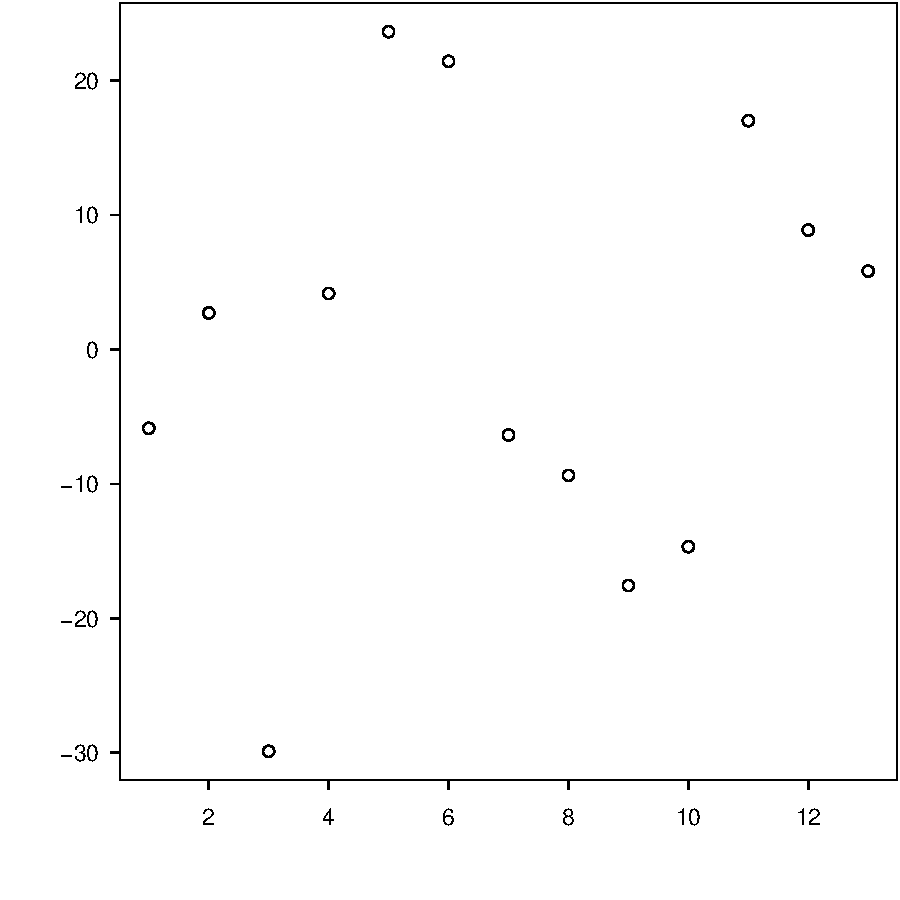
\includegraphics[width=.6\linewidth]{figure/problem-3-mid-term-Rnwauto-report-1} 

}


\begin{kframe}\begin{alltt}
\hlcom{# second residuals plot }

\hlkwd{residuals}\hlstd{(reg_2)}
\end{alltt}
\begin{verbatim}
##          1          2          3          4          5          6          7          8 
##  -7.077558   4.110066 -29.290924   3.147690  26.446205  20.622937  -9.589439  -9.392739 
##          9         10         11         12         13 
## -15.772772 -13.081353  12.774917  10.276733   6.826238
\end{verbatim}
\begin{alltt}
\hlkwd{plot}\hlstd{(}\hlkwd{residuals}\hlstd{(reg_2),}\hlkwc{xlab}\hlstd{=}\hlstr{" "}\hlstd{,}\hlkwc{ylab}\hlstd{=}\hlstr{" "}\hlstd{,}\hlkwc{main}\hlstd{=)}
\end{alltt}
\end{kframe}

{\centering 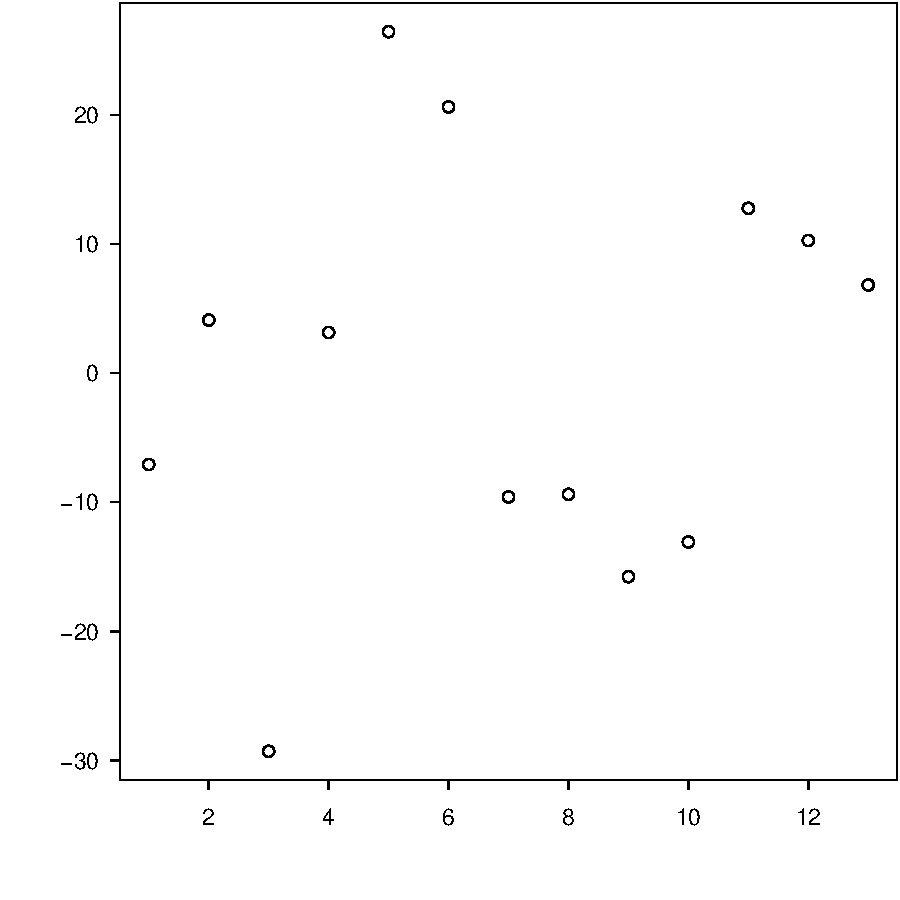
\includegraphics[width=.6\linewidth]{figure/problem-3-mid-term-Rnwauto-report-2} 

}


\begin{kframe}\begin{alltt}
\hlcom{# third residuals plot }

\hlkwd{residuals}\hlstd{(reg_3)}
\end{alltt}
\begin{verbatim}
##          1          2          3          4          5          6          7          8 
##  -7.781301   7.452846 -22.781301   1.652236  38.585772  18.335772 -16.714837 -14.846748 
##          9         10         11         12         13 
## -14.013415 -10.530285  -4.730691  13.619512  11.752439
\end{verbatim}
\begin{alltt}
\hlkwd{plot}\hlstd{(}\hlkwd{residuals}\hlstd{(reg_3),}\hlkwc{xlab}\hlstd{=}\hlstr{" "}\hlstd{,}\hlkwc{ylab}\hlstd{=}\hlstr{" "}\hlstd{,}\hlkwc{main}\hlstd{=)}
\end{alltt}
\end{kframe}

{\centering 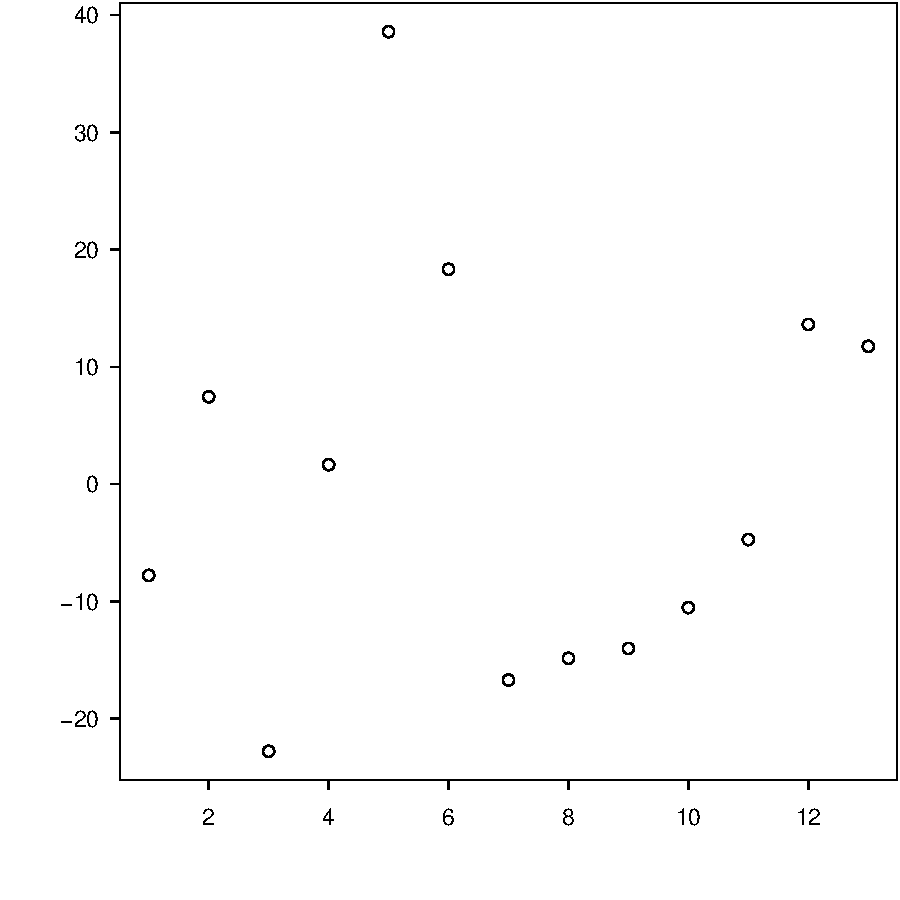
\includegraphics[width=.6\linewidth]{figure/problem-3-mid-term-Rnwauto-report-3} 

}


\begin{kframe}\begin{alltt}
\hlcom{# hypothesis testing and confidence interval for beta_2}

\hlstd{n}\hlkwb{=} \hlnum{13}

\hlstd{beta_hat_2} \hlkwb{=} \hlnum{111111111111111111111}

\hlstd{se} \hlkwb{=} \hlnum{111111111111}

\hlstd{t_statistics} \hlkwb{=} \hlkwd{qt}\hlstd{(}\hlnum{1}\hlopt{-}\hlnum{0.05}\hlopt{/}\hlnum{2}\hlstd{,} \hlkwc{df}\hlstd{=n}\hlopt{-}\hlnum{3}\hlstd{)}  \hlcom{# 95% CI}
\hlkwd{c}\hlstd{(betahat1}\hlopt{-}\hlstd{t_statistics}\hlopt{*}\hlstd{se, betahat1}\hlopt{+}\hlstd{t_statistics}\hlopt{*}\hlstd{se)}
\end{alltt}


{\ttfamily\noindent\bfseries\color{errorcolor}{\#\# Error in eval(expr, envir, enclos): object 'betahat1' not found}}\end{kframe}
\end{knitrout}

The R session information (including the OS info, R version and all
packages used):

\begin{knitrout}
\definecolor{shadecolor}{rgb}{0.969, 0.969, 0.969}\color{fgcolor}\begin{kframe}
\begin{alltt}
\hlkwd{sessionInfo}\hlstd{()}
\end{alltt}
\begin{verbatim}
## R version 4.0.3 (2020-10-10)
## Platform: x86_64-w64-mingw32/x64 (64-bit)
## Running under: Windows 10 x64 (build 19042)
## 
## Matrix products: default
## 
## locale:
## [1] LC_COLLATE=English_United States.1252  LC_CTYPE=English_United States.1252   
## [3] LC_MONETARY=English_United States.1252 LC_NUMERIC=C                          
## [5] LC_TIME=English_United States.1252    
## 
## attached base packages:
## [1] stats     graphics  grDevices utils     datasets  methods   base     
## 
## other attached packages:
## [1] tidyr_1.1.3    dplyr_1.0.6    readxl_1.3.1   ggplot2_3.3.3  deBInfer_0.4.2
## [6] deSolve_1.28  
## 
## loaded via a namespace (and not attached):
##  [1] tinytex_0.29       tidyselect_1.1.1   xfun_0.26          purrr_0.3.4       
##  [5] lattice_0.20-41    colorspace_2.0-1   vctrs_0.3.8        generics_0.1.0    
##  [9] testthat_3.0.2     htmltools_0.5.1.1  stats4_4.0.3       utf8_1.1.4        
## [13] rlang_0.4.10       pillar_1.6.1       glue_1.4.2         withr_2.4.1       
## [17] DBI_1.1.1          RColorBrewer_1.1-2 lifecycle_1.0.0    plyr_1.8.6        
## [21] stringr_1.4.0      munsell_0.5.0      gtable_0.3.0       cellranger_1.1.0  
## [25] bayestestR_0.11.0  mvtnorm_1.1-1      coda_0.19-4        evaluate_0.14     
## [29] knitr_1.36         datawizard_0.2.1   fansi_0.4.2        evd_2.3-3         
## [33] highr_0.8          Rcpp_1.0.6         scales_1.1.1       desc_1.2.0        
## [37] pkgload_1.1.0      PBSddesolve_1.12.6 digest_0.6.27      stringi_1.5.3     
## [41] insight_0.14.4     grid_4.0.3         rprojroot_2.0.2    cli_2.5.0         
## [45] tools_4.0.3        magrittr_2.0.1     tibble_3.1.2       crayon_1.4.1      
## [49] pkgconfig_2.0.3    MASS_7.3-54        ellipsis_0.3.2     truncdist_1.0-2   
## [53] correlation_0.7.1  assertthat_0.2.1   rmarkdown_2.6      rstudioapi_0.13   
## [57] R6_2.5.0           compiler_4.0.3
\end{verbatim}
\begin{alltt}
\hlkwd{Sys.time}\hlstd{()}
\end{alltt}
\begin{verbatim}
## [1] "2021-10-16 11:11:46 CDT"
\end{verbatim}
\end{kframe}
\end{knitrout}


\end{document}
